\documentclass[a4paper,10pt]{article}
\usepackage[utf8]{inputenc}
\usepackage{graphicx}
\usepackage[thinlines]{easytable}
\usepackage{enumitem}
\usepackage{amsmath}
%opening
\title{Force Control on a Wheeled Inverted Pendulum Robot}
\author{Munzir Zafar}

\begin{document}

\maketitle

\begin{abstract}

\end{abstract}

\section{Problem Definition}

\begin{figure}[!ht]
\centering 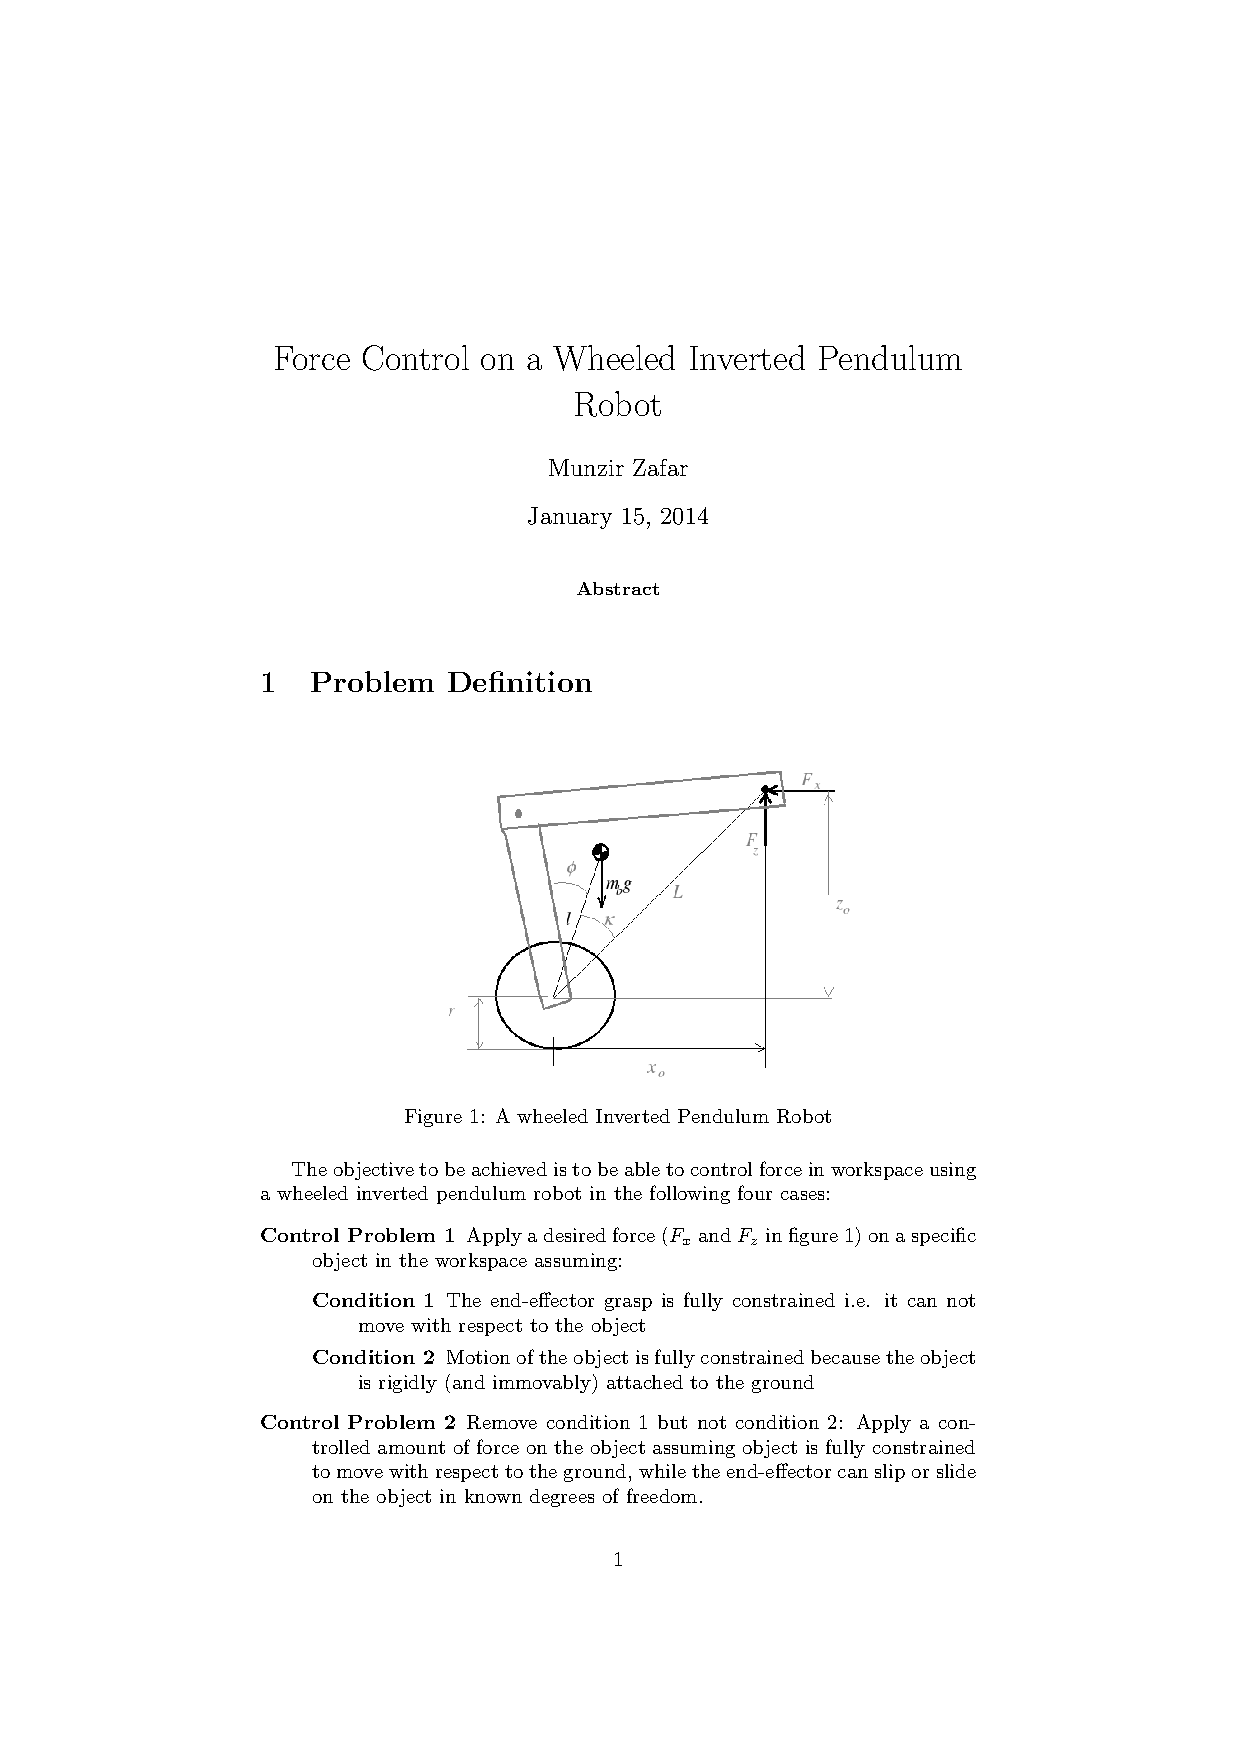
\includegraphics[width=1.0\columnwidth]{/home/munzir/Desktop/forceBalance.png}
\caption{A wheeled Inverted Pendulum Robot}
\label{fig:model} 
\end{figure}

The objective to be achieved is to be able to control force in workspace using a wheeled inverted pendulum
robot in the following four cases:

\begin{description}
 \item[Control Problem 1] Apply a desired force ($F_x$ and $F_z$ in figure \ref{fig:model}) on a specific object in the 
 workspace assuming:
 \begin{description}
  \item[Condition 1] The end-effector grasp is fully constrained i.e. it can not move with respect to the object
  \item[Condition 2] Motion of the object is fully constrained 
  because the object is rigidly (and immovably) attached to the ground 
 \end{description}
 \item[Control Problem 2] Remove condition 1 but not condition 2: Apply a controlled amount of force on the object
 assuming object is fully constrained to move with respect to the ground, while the end-effector can slip or slide on the object 
 in known degrees of freedom.
 \item[Control Problem 3] Remove condition 2 but not condition 1: Move the object in a specified trajectory assuming that the end-effector
 is still fully constrained to move with respect to the object, while the the object can move in the workspace under known
 kinematic constraints. 
 
 \textit{Additional condition}: The object will only begin (and continue) to move when a large amount of 
 resistance is overcome. This requires a constant application of a controlled force on the moving object through the trajectory.
 \item[Control Problem 4] Remove both conditions 1 and 2. Move the object in a specified trajectory assuming the object can move in the workspace 
 under known kinematic constraints and that the end-effector can move with respect to the object in known
 degrees of freedom. The additional condition of control problem 3
 is also assumed to be applicable.
\end{description}

\section{System Model}
We understand the dynamics of a wheeled inverted pendulum robot to be governed by two equations:
{\small
\begin{align}
 \tau - \tau_f - F_x r = \lbrack(m_b + m_w)r^2 + I_w + \eta^2 I\rbrack\ddot{\theta} + (m_brlcos\theta -\eta^2I_m)\ddot{\phi}&\nonumber \\
 - m_brl\dot{\phi}^2 sin\phi& \\
 \tau - \tau_f + F_x L cos(\phi+\kappa) + F_z L sin(\phi+\kappa) - mglsin\phi = (\eta^2I_m - m_brlcos\phi)\ddot{\theta}&  \nonumber \\
 - (m_bl^2+I_b+\eta^2I_m)\ddot{\phi}&
\end{align}
}

where $\tau$, $I$ and $\eta$ are wheel motor's torque, inertia and gear-ratio respectively. $\tau_f$, $m_w$, $I_w$ and $\theta$ are
wheel friction, mass, inertia and rotation respectively. All other variables are shown in figure \ref{fig:model}.

\section{Control Problem 1}
Under the conditions of fully constrained object and end-effector, and a given pose of the robot
we can safely assume that the system will retain its configuration under all circumstances. That is
the wheels will stay steady without the need of any intelligent control. The position of the wheels and the center 
of mass of the robot will be determined by the geometric constraint:
\[
  Lsin(\phi+\kappa) = x_o 
\]
Given a specific position of object in the workspace ($x_o = const$) and a specific pose of the robot ($L$ and $\kappa$)
the location of the center of mass of the robot is fixed ($\dot\phi = \ddot\phi = 0$). Similarly the wheels
of the robot can also not move ($\dot\theta = \ddot\theta = 0$), as any motion of the wheels would either lead to a motion of the end-effector or 
the object which are both fully constrained. In this situation, the dynamic equations of the system reduce to:

\begin{align}
 \tau - F_xr &= 0 \\
 \tau + F_xLcos(\phi+\kappa) + F_zLsin(\phi+\kappa) - m_bglsin\phi &= 0 \label{eq:FLinDep}
\end{align}

Also, this means that there is no need for any balancing controller to keep the robot balanced as the robot is not
going to move in this case. Based on the equations we can see that for a given torque $\tau$ of the wheel motors, 
the forces $F_x$ and $F_z$ are linearly dependent as determined by equation \ref{eq:FLinDep}, which has parameters
$\tau$, $m_b$, $\phi$, $l$, $L$ and $\kappa$. Of these, $\tau$ is the control input that we will choose as 
$F_xr$ while the last four parameters are functions of the pose $q$ of the robot. This means that for a given pose,
using the control input $\tau$, both $F_x$ and $F_z$ can not be controlled independently. It may, however, be possible to achieve 
independent control of both $F_x$ and $F_z$ by varying the pose of the robot.

\subsection{Controlling Pose For Independent Force Control}

We can re-write equation \ref{eq:FLinDep} such that it simplifies the relationship of the $q$ to
the forces experienced at the end-effector in steady state. Noting that $Lcos(\phi+\kappa) = z_o$,
$Lsin(\phi+\kappa) = x_o$, $lsin\phi = x_{COG} = $ the x-coordinate of the COG and that $\tau = F_xr$
equation \ref{eq:FLinDep} becomes:
\begin{align}
 F_xr + F_xz_o + F_zx_o - m_bgx_{COG} &= 0 \nonumber \\
 m_bgx_{COG}(q) - F_zx_o(q) &= F_x (r + z_o) \label{eq:constraintOnQ}
\end{align}

From this expression we deduce that all we need to do in order to be able to control the forces
independently is to control the pose $q$ to move $x_{COG}$ and $x_o$ to values that satisfy equation
\ref{eq:constraintOnQ} while maintainig the orientation and $y$, $z$ coordinates of the end-effector
in the workspace. So control of $x_{COG}$ and $x_o$ can take place in the null-space of the
workspace position controller of the end-effector. This position controller however is using
the jacobians with repect to all body joints rather than just the joints up till the shoulder.

\subsection{Planning}
The following steps need to be undertaken:
\begin{description}
 \item[01/15] \hfill \\
 Write expression for the control law and the Jacobians for $x_{COG}$ and $x_o$. Make an experimental
 setup for control problem 1. And try to control just $F_x$ using $\tau$
 \item[01/16-18] \hfill \\
 Write the agorithm for realizing the control strategy discussed
 \item[01/20 onwards] \hfill \\
 Experimentation and Results. If successful, think about strategies to tackle control problems 2-4.
\end{description}

\end{document}
